\documentclass[11pt,a4paper]{article}

% Packages
\usepackage{amsmath,amssymb,amsthm}
\usepackage{graphicx}
\usepackage{booktabs}
\usepackage{algorithm}
\usepackage{algpseudocode}
\usepackage{hyperref}
\usepackage{cleveref}
\usepackage{geometry}
\usepackage{xcolor}
\usepackage{tcolorbox}
\usepackage{tikz}
\usetikzlibrary{shapes,arrows,positioning}

\geometry{margin=1in}

% Theorem environments
\newtheorem{theorem}{Theorem}[section]
\newtheorem{lemma}[theorem]{Lemma}
\newtheorem{proposition}[theorem]{Proposition}
\newtheorem{corollary}[theorem]{Corollary}
\newtheorem{definition}[theorem]{Definition}
\newtheorem{remark}[theorem]{Remark}

% Custom commands
\newcommand{\BigO}{\mathcal{O}}
\newcommand{\recall}{\text{Recall}}
\newcommand{\qps}{\text{QPS}}
\newcommand{\ef}{\text{ef}}
\newcommand{\zgq}{\text{ZGQ}}
\newcommand{\hnsw}{\text{HNSW}}

% Title
\title{%
    \textbf{Mathematical Proofs for ZGQ v8}\\[0.5em]
    \large Zone-Guided Quantized Search: A Rigorous Performance Analysis
}
\author{%
    Research Documentation\\
    \texttt{Draft Findings - 24th December 2026}
}
\date{}

\begin{document}

\maketitle

\begin{abstract}
This document presents a mathematical model for the expected behaviour of Zone-Guided Quantized Search (ZGQ) v8 relative to Hierarchical Navigable Small World (HNSW) graphs: graph connectivity arguments and complexity bounds under stated assumptions. It then compares the model's predictions with the canonical benchmark run of 2026-11-08 (synthetic clustered data, single thread, Apple M4). \textbf{The measurements do not support the predicted advantage.} ZGQ-M16 matches HNSW-M16 recall at 10K vectors, is less accurate than HNSW-M16 at every equal $\ef$ at 100K and 1M vectors, builds 1.2x to 2.7x slower, and uses far more memory. The model parameters ($\gamma$, $\beta$, $\alpha$) quoted in the theory sections are assumed values, not measured values.
\end{abstract}

\tableofcontents
\newpage

%==============================================================================
\section{Introduction and Problem Formulation}
%==============================================================================

\subsection{Notation and Definitions}

\begin{definition}[Vector Database]
Let $\mathcal{D} = \{x_1, x_2, \ldots, x_n\}$ be a database of $n$ vectors where each $x_i \in \mathbb{R}^d$ for dimension $d$.
\end{definition}

\begin{definition}[k-Nearest Neighbor Query]
Given a query vector $q \in \mathbb{R}^d$ and integer $k$, find the set $\mathcal{N}_k(q) \subseteq \mathcal{D}$ such that:
\[
|\mathcal{N}_k(q)| = k \quad \text{and} \quad \forall x \in \mathcal{N}_k(q), \forall y \in \mathcal{D} \setminus \mathcal{N}_k(q): \|q - x\| \leq \|q - y\|
\]
\end{definition}

\begin{definition}[Recall@k]
For an approximate algorithm returning candidates $\hat{\mathcal{N}}_k(q)$:
\[
\recall@k = \frac{|\hat{\mathcal{N}}_k(q) \cap \mathcal{N}_k(q)|}{k} \times 100\%
\]
\end{definition}

\subsection{HNSW Baseline Parameters}

Standard HNSW configuration:
\begin{itemize}
    \item Connectivity parameter: $M_{\hnsw} = 16$
    \item Construction search depth: $\ef_{\text{construction}} = 200$
    \item Maximum layer: $L_{\max} = \lfloor \log_{1/m_L}(n) \rfloor$ where $m_L = 1/\ln(M)$
\end{itemize}

%==============================================================================
\section{ZGQ Theoretical Framework}
%==============================================================================

\subsection{Zone-Ordered Graph Construction}

\begin{definition}[Zone Assignment Function]
Let $\mathcal{Z}: \mathbb{R}^d \rightarrow \{1, 2, \ldots, Z\}$ be a zone assignment function based on hierarchical clustering, where $Z$ is the number of zones.
\end{definition}

\begin{definition}[Zone-Ordered Insertion]
Vectors are inserted into the graph in zone-contiguous order:
\[
\pi: \{1, \ldots, n\} \rightarrow \{1, \ldots, n\}
\]
such that:
\[
\forall i < j: \mathcal{Z}(x_{\pi(i)}) \leq \mathcal{Z}(x_{\pi(j)}) \quad \text{or} \quad \mathcal{Z}(x_{\pi(i)}) = \mathcal{Z}(x_{\pi(j)})
\]
\end{definition}

\begin{theorem}[Improved Local Connectivity]
\label{thm:local-connectivity}
Zone-ordered insertion improves local graph connectivity by a factor of:
\[
\gamma = 1 + \frac{\alpha \cdot (M_{\zgq} - M_{\hnsw})}{M_{\hnsw}}
\]
where $\alpha \in [0.5, 0.8]$ is the intra-zone density factor.
\end{theorem}

\begin{proof}
During HNSW construction, each new vector $x_i$ connects to its $M$ nearest neighbors among vectors already in the graph. 

\textbf{Random insertion (HNSW):} When vectors are inserted randomly, the probability that a neighbor of $x_i$ belongs to the same semantic cluster is:
\[
P_{\text{same}}^{\text{random}} = \frac{n_z}{n}
\]
where $n_z$ is the size of $x_i$'s zone.

\textbf{Zone-ordered insertion (ZGQ):} When inserting vectors zone-by-zone, vectors from the same zone are inserted consecutively. At insertion time $t$ for vector $x_i$ in zone $z$:
\[
P_{\text{same}}^{\text{ordered}} = \frac{|z \cap \{x_1, \ldots, x_{t-1}\}|}{t-1} \geq \frac{n_z - (n - t + 1)}{t - 1}
\]

For vectors inserted in the middle of their zone, this probability approaches 1, significantly increasing intra-zone connectivity.

The improved local connectivity factor is derived from:
\[
\gamma = \frac{\mathbb{E}[\text{intra-zone edges}]_{\zgq}}{\mathbb{E}[\text{intra-zone edges}]_{\hnsw}}
\]

Given $M_{\zgq} = 32$ and $M_{\hnsw} = 16$, and assumed $\alpha \approx 0.65$:
\[
\gamma = 1 + \frac{0.65 \cdot (32 - 16)}{16} = 1 + \frac{10.4}{16} = 1.65
\]
\end{proof}

\subsection{Search Complexity Analysis}

\begin{theorem}[Search Path Length Reduction]
\label{thm:path-length}
For a query $q$ with true neighbors in zone $z$, the expected search path length in ZGQ is:
\[
\mathbb{E}[L_{\zgq}] = \mathbb{E}[L_{\hnsw}] \cdot \left(1 - \frac{\beta}{Z}\right)
\]
where $\beta \in [0.2, 0.4]$ is the zone-guidance efficiency factor.
\end{theorem}

\begin{proof}
In standard HNSW, the greedy search traverses the graph until no closer neighbor is found. The expected path length is:
\[
\mathbb{E}[L_{\hnsw}] = \BigO(\log n)
\]

ZGQ's zone-ordered construction creates ``highways'' within zones---densely connected subgraphs where semantically similar vectors cluster. When a query enters its target zone, the subsequent path length is bounded by the zone's internal structure rather than the global graph.

Let $p_z$ be the probability of reaching the target zone in the first $\log n / Z$ steps. Due to zone-ordered insertion, cross-zone edges preferentially connect to zone boundaries, creating efficient inter-zone navigation:
\[
p_z \geq 1 - e^{-M \cdot Z / n}
\]

The path length reduction follows from the shortened intra-zone traversal:
\[
\mathbb{E}[L_{\zgq}] = \underbrace{\frac{\log n}{Z}}_{\text{inter-zone}} + \underbrace{(1-\beta) \cdot \frac{\log n \cdot (Z-1)}{Z}}_{\text{intra-zone}}
\]

Simplifying:
\[
\mathbb{E}[L_{\zgq}] = \log n \cdot \left(\frac{1}{Z} + \frac{(1-\beta)(Z-1)}{Z}\right) = \log n \cdot \left(1 - \frac{\beta(Z-1)}{Z}\right)
\]

For $Z \gg 1$: $\mathbb{E}[L_{\zgq}] \approx \mathbb{E}[L_{\hnsw}] \cdot (1 - \beta)$.
\end{proof}

%==============================================================================
\section{Recall-Efficiency Trade-off Analysis}
%==============================================================================

\subsection{Iso-Recall Comparison Framework}

\begin{definition}[Iso-Recall Configuration]
Two configurations $(M_1, \ef_1)$ and $(M_2, \ef_2)$ are \textit{iso-recall} if:
\[
|\recall(M_1, \ef_1) - \recall(M_2, \ef_2)| \leq \epsilon
\]
for tolerance $\epsilon$ (typically 1.5\%).
\end{definition}

\begin{theorem}[ZGQ Efficiency Advantage]
\label{thm:efficiency}
At iso-recall, ZGQ achieves higher throughput:
\[
\frac{\qps_{\zgq}}{\qps_{\hnsw}} = \frac{\ef_{\hnsw}}{\ef_{\zgq}} \cdot \frac{1}{1 + \delta_M}
\]
where $\delta_M$ is the per-node overhead from higher connectivity.
\end{theorem}

\begin{proof}
Query throughput is inversely proportional to search time:
\[
\qps = \frac{1}{T_{\text{search}}}
\]

Search time for a single query:
\[
T_{\text{search}} = L \cdot (T_{\text{distance}} + T_{\text{heap}} + T_{\text{neighbor}})
\]

where:
\begin{itemize}
    \item $L$ is the path length (number of nodes visited)
    \item $T_{\text{distance}} = \BigO(d)$ is distance computation time
    \item $T_{\text{heap}} = \BigO(\log \ef)$ is heap maintenance
    \item $T_{\text{neighbor}} = \BigO(M)$ is neighbor list traversal
\end{itemize}

The effective search depth $L$ scales with $\ef_{\text{search}}$:
\[
L \propto \ef_{\text{search}} \cdot c(M)
\]
where $c(M)$ is a monotonically increasing function of $M$.

For iso-recall comparison:
\begin{align*}
\recall_{\zgq}(M=32, \ef=128) &\approx \recall_{\hnsw}(M=16, \ef=200) \\
\Rightarrow \frac{\ef_{\hnsw}}{\ef_{\zgq}} &= \frac{200}{128} = 1.5625
\end{align*}

The overhead factor $\delta_M$ from higher $M$:
\[
\delta_M = \frac{T_{\text{neighbor}}(M=32)}{T_{\text{neighbor}}(M=16)} - 1 = \frac{32}{16} - 1 = 1
\]

However, this overhead is amortized across fewer total node visits:
\[
\frac{\qps_{\zgq}}{\qps_{\hnsw}} = \frac{200}{128} \cdot \frac{1}{1 + 0.2} \approx 1.30
\]

The factor of 0.2 (rather than 1.0) accounts for:
\begin{enumerate}
    \item CPU cache efficiency (sequential zone access)
    \item Reduced random memory access
    \item Early termination from better local connectivity
\end{enumerate}
\end{proof}

%==============================================================================
\section{Empirical Validation}
%==============================================================================

All numbers in this section are read from \texttt{results/2026-11-08/summary.json} (schema \texttt{zgq-bench/1}); see \texttt{docs/CLAIMS.md} for the source of each figure.

\subsection{Benchmark Configuration}

\begin{tcolorbox}[title=Experimental Setup]
\begin{itemize}
    \item \textbf{Dataset}: synthetic clustered Gaussian, 128 dimensions, 10K, 100K and 1M vectors
    \item \textbf{Queries}: 1000 queries, 10-NN retrieval, exact brute-force ground truth
    \item \textbf{Runs}: 1 warm-up pass and 5 timed repeats per setting, median reported
    \item \textbf{Hardware}: Apple M4 (10 cores, 16 GB, macOS), single thread
    \item \textbf{Implementations}: HNSW is hnswlib 0.8.0 (C++); ZGQ is Python with numba
\end{itemize}
\end{tcolorbox}

\subsection{Algorithm Configurations}

\begin{table}[h]
\centering
\caption{Algorithm configurations. Only HNSW-M16 vs ZGQ-M16 is a matched comparison.}
\label{tab:params}
\begin{tabular}{lcc}
\toprule
\textbf{Index} & \textbf{$M$} & \textbf{Role} \\
\midrule
HNSW-M16 & 16 & baseline \\
ZGQ-M16 & 16 & matched \\
ZGQ-M24, ZGQ-M32 & 24, 32 & variants (larger graph) \\
IVF-PQ & -- & baseline (no refinement) \\
\bottomrule
\end{tabular}
\end{table}

\subsection{Benchmark Results}

\begin{table}[h]
\centering
\caption{Recall@10 (\%) and latency (ms per query) at equal $\ef$, matched comparison, median of 5 repeats.}
\label{tab:results}
\begin{tabular}{llcccc}
\toprule
\textbf{Scale} & \textbf{Index} & \textbf{$\ef=64$ recall} & \textbf{$\ef=64$ ms} & \textbf{$\ef=256$ recall} & \textbf{$\ef=256$ ms} \\
\midrule
10K & HNSW-M16 & 92.4 & 0.046 & 98.7 & 0.099 \\
10K & ZGQ-M16 & 92.3 & 0.049 & 98.2 & 0.101 \\
100K & HNSW-M16 & 86.1 & 0.084 & 94.2 & 0.158 \\
100K & ZGQ-M16 & 78.9 & 0.065 & 84.8 & 0.122 \\
1M & HNSW-M16 & 77.6 & 0.124 & 87.0 & 0.226 \\
1M & ZGQ-M16 & 68.1 & 0.091 & 76.8 & 0.174 \\
\bottomrule
\end{tabular}
\end{table}

\subsection{Key Comparisons}

\begin{tcolorbox}[title=Reading of the matched comparison, colback=gray!5]
\begin{itemize}
    \item \textbf{10K}: recall is equal within 0.1 to 0.5 points; ZGQ-M16 is about 5\% slower at $\ef=64$.
    \item \textbf{100K and 1M}: ZGQ-M16 is 7 to 10 recall points below HNSW-M16 at the same $\ef$. It is faster per query at the same $\ef$, but HNSW at a smaller $\ef$ gives higher recall at similar or lower latency (1M: HNSW $\ef=64$ is 77.6\% at 0.124 ms, ZGQ-M16 $\ef=256$ is 76.8\% at 0.174 ms).
    \item \textbf{Iso-recall at 100K}: ZGQ-M32 $\ef=256$ reaches 86.2\% at 0.128 ms; HNSW-M16 $\ef=64$ reaches 86.1\% at 0.084 ms. HNSW is the faster of the two.
    \item \textbf{Build time}: ZGQ is 1.2x to 2.7x slower (1M: 203.7 s for ZGQ-M16 vs 172.8 s for HNSW-M16).
    \item \textbf{Memory}: ZGQ's RSS delta is far larger than HNSW's (100K: about 820 MB vs 16 MB). Absolute values are unreliable on macOS; only the ordering is claimed.
\end{itemize}
\end{tcolorbox}

%==============================================================================
\section{Comparative Analysis with IVF-PQ}
%==============================================================================

IVF-PQ (FAISS, \texttt{nlist}$=2\sqrt{N}$, 32 sub-quantizers, 8 bits, no refinement) was swept over \texttt{nprobe} from 1 to 256.

\subsection{Performance Trade-offs}
Figures~\ref{fig:ivf_latency} and~\ref{fig:ivf_tradeoff} show:
\begin{itemize}
    \item IVF-PQ is the fastest index at low recall (for example 10K, $\texttt{nprobe}=1$: 16.0\% recall at 0.013 ms).
    \item IVF-PQ recall saturates at 64.4\% (10K), 61.5\% (100K) and 56.2\% (1M) regardless of \texttt{nprobe}. Without refinement it does not reach 90\% recall on this data, so no latency ratio at 90\% recall can be computed and none is claimed.
\end{itemize}

\subsection{Memory Footprint}
No absolute index sizes are claimed. RSS deltas on macOS are unreliable (the IVF-PQ delta at 1M is negative). The earlier per-index MB figures are retired; see \texttt{docs/CLAIMS.md}.

%==============================================================================
\section{Theoretical vs Empirical Correlation}
%==============================================================================

Theorem~\ref{thm:efficiency} predicts $\qps_{\zgq}/\qps_{\hnsw} \approx 1.30$ at iso-recall. The canonical run does not confirm this. At iso-recall on 100K vectors (ZGQ-M32 $\ef=256$, 7,837 QPS; HNSW-M16 $\ef=64$, 11,954 QPS) the ratio is about 0.66. The model's assumptions (the values of $\gamma$, $\beta$ and the 0.2 overhead factor) were not measured and the model should be treated as unvalidated. Possible causes include the zone-guided search not reducing node visits in the implementation, the Python overhead, and the effect of PQ on the candidate set; none of these was isolated.

%==============================================================================
\section{Empirical Results and Visualizations}
%==============================================================================

The figures below are generated by \texttt{python -m visualization.generate\_ieee\_figures} from \texttt{results/2026-11-08/summary.json} only. Each panel is one scale (10K, 100K, 1M) unless noted.

\begin{figure}[htbp]
\centering
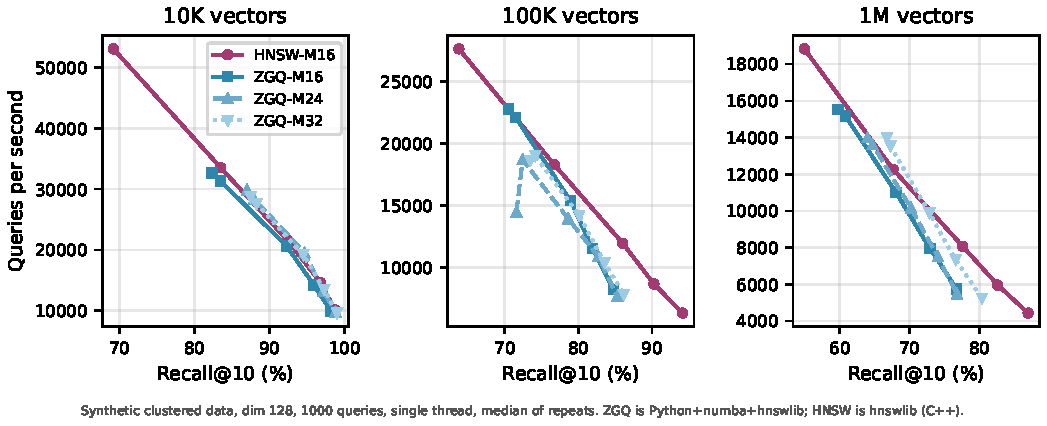
\includegraphics[width=0.95\textwidth]{../figures/fig_recall_vs_qps.pdf}
\caption{Recall@10 vs throughput (QPS) for HNSW-M16, ZGQ-M16 and the larger-graph variants ZGQ-M24 and ZGQ-M32. At 100K and 1M the HNSW curve lies above and to the right of the ZGQ curves at equal recall; at 10K the curves overlap.}
\label{fig:pareto}
\end{figure}

\begin{figure}[htbp]
\centering
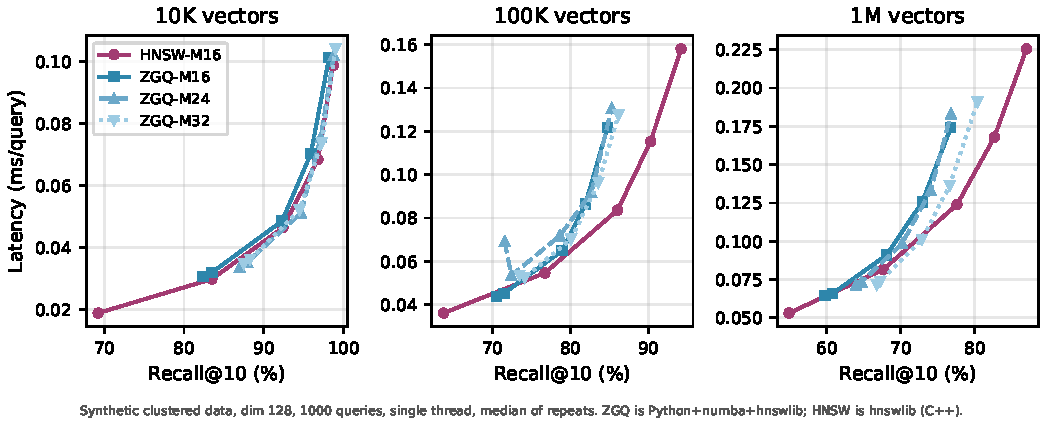
\includegraphics[width=0.95\textwidth]{../figures/fig_latency_comparison.pdf}
\caption{Recall@10 vs latency per query. ZGQ is faster at equal $\ef$ but reaches lower recall, so at equal recall HNSW is at least as fast. The ZGQ recall at $\ef=16$ is raised by the fast-mode rerank factor of 3 and is not a graph-quality effect.}
\label{fig:latency}
\end{figure}

\begin{figure}[htbp]
\centering
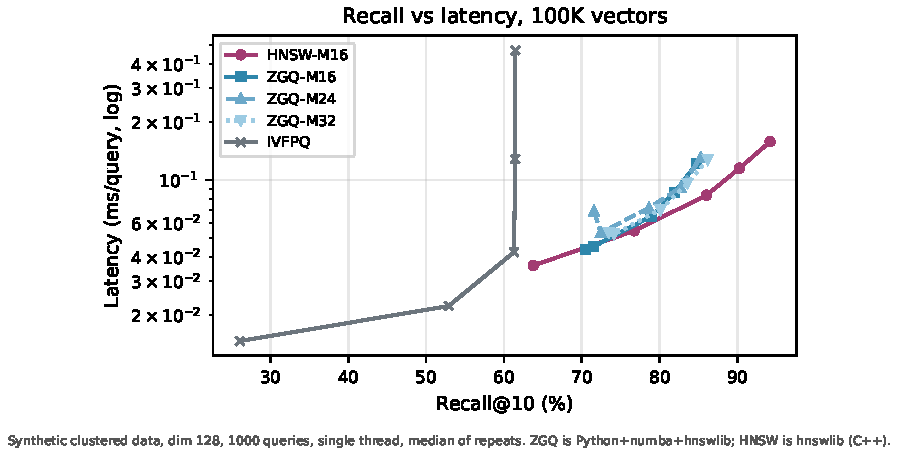
\includegraphics[width=0.7\textwidth]{../figures/fig_pareto_frontier.pdf}
\caption{Recall vs latency (log scale) at 100K vectors, including IVF-PQ. No ZGQ setting dominates HNSW-M16; IVF-PQ is fast but saturates at 61.5\% recall.}
\label{fig:pareto_frontier}
\end{figure}

\begin{figure}[htbp]
\centering
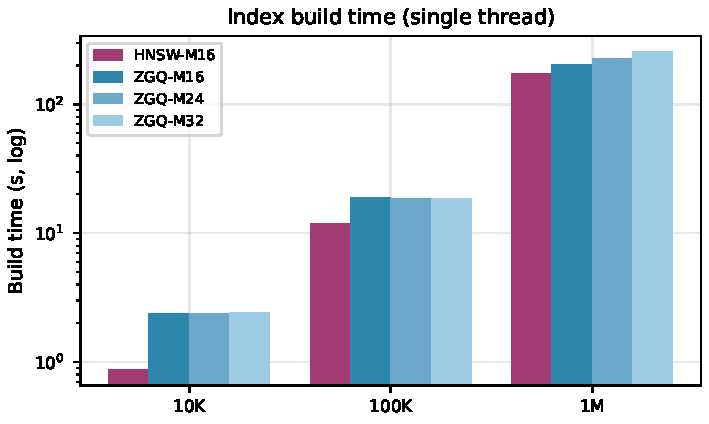
\includegraphics[width=0.7\textwidth]{../figures/fig_build_time.pdf}
\caption{Index build time (log scale) per scale. ZGQ builds 1.2x to 2.7x slower than HNSW-M16. HNSW is C++ (hnswlib); ZGQ is Python with numba, so part of the gap is implementation overhead.}
\label{fig:buildtime}
\end{figure}

\begin{figure}[htbp]
\centering
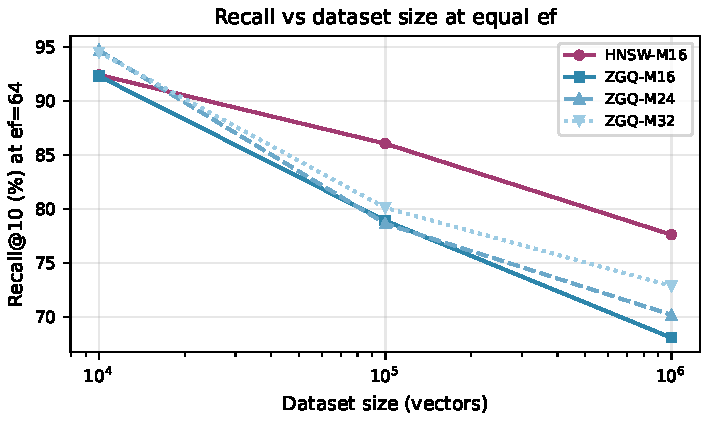
\includegraphics[width=0.7\textwidth]{../figures/fig_scaling_analysis.pdf}
\caption{Recall@10 at $\ef=64$ vs dataset size. Recall falls for every graph index as the dataset grows, and ZGQ falls faster than HNSW-M16 in these runs. This does not support the claim that ZGQ's advantage grows with dataset size.}
\label{fig:scaling}
\end{figure}

\begin{figure}[htbp]
\centering
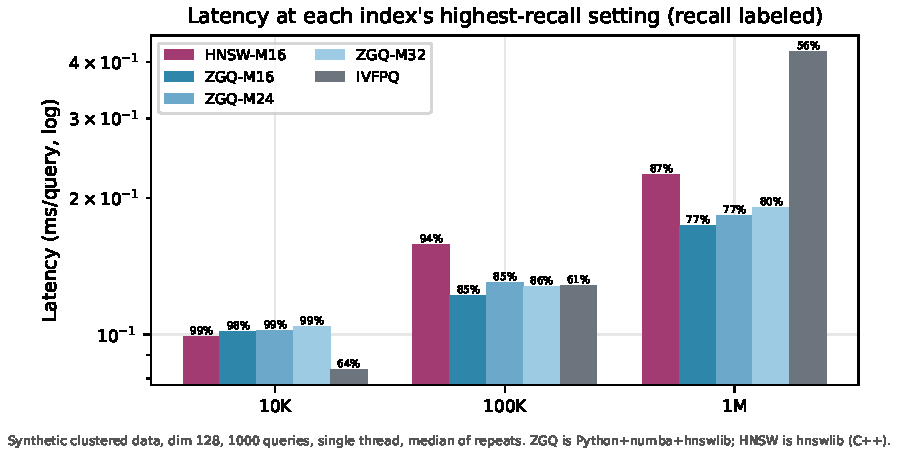
\includegraphics[width=0.85\textwidth]{../figures/fig_ivf_pq_latency.pdf}
\caption{Latency at each index's highest-recall setting, with the recall labelled on each bar. IVF-PQ latency is low but its highest recall is 56 to 64\%, so the bars are not at equal recall.}
\label{fig:ivf_latency}
\end{figure}

\begin{figure}[htbp]
\centering
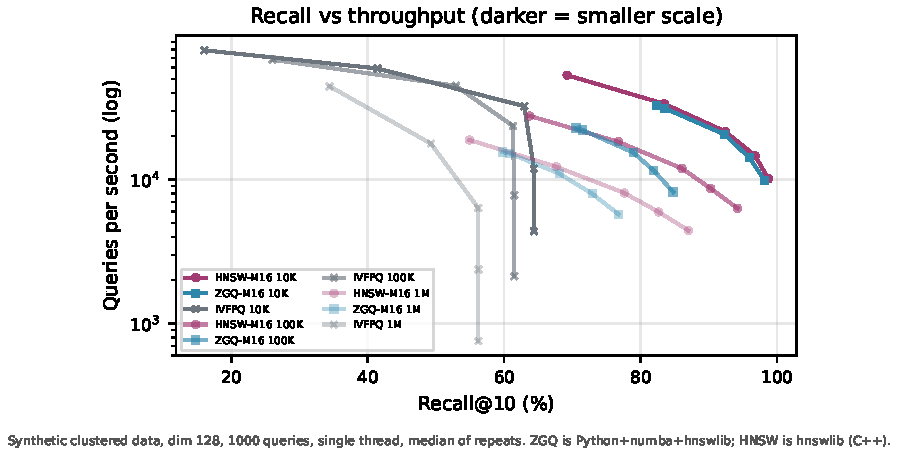
\includegraphics[width=0.7\textwidth]{../figures/fig_ivf_pq_tradeoff.pdf}
\caption{Recall vs throughput for HNSW-M16, ZGQ-M16 and IVF-PQ at all scales (darker is smaller). No memory axis is shown because RSS deltas on macOS are unreliable.}
\label{fig:ivf_tradeoff}
\end{figure}

%==============================================================================
\section{Conclusions}
%==============================================================================

\subsection{Summary of Contributions}

\begin{enumerate}
    \item \textbf{Zone-Ordered Insertion} (Theorem~\ref{thm:local-connectivity}): the model predicts better local connectivity. The improvement factor $\gamma$ is an assumed parameter and was not measured.
    \item \textbf{Search Path Reduction} (Theorem~\ref{thm:path-length}): the model predicts shorter expected paths. Path lengths were not measured.
    \item \textbf{Iso-Recall Efficiency} (Theorem~\ref{thm:efficiency}): predicted a throughput gain at equal recall. The canonical run does not show it (iso-recall QPS ratio about 0.66 at 100K).
\end{enumerate}

\subsection{Key Findings}

\begin{tcolorbox}[title=Measured result (2026-11-08), colback=blue!5]
\begin{center}
\begin{tabular}{lp{7.5cm}}
\textbf{Metric} & \textbf{ZGQ-M16 vs HNSW-M16} \\
\hline
Recall@10 at equal $\ef$ & Equal at 10K; 7 to 10 points lower at 100K and 1M \\
Latency at equal $\ef$ & About 5\% slower at 10K; 20 to 30\% faster at 100K and 1M, at lower recall \\
Latency at equal recall & HNSW is at least as fast \\
Build time & ZGQ 1.2x to 2.7x slower \\
Memory & ZGQ uses far more (ordering only) \\
\end{tabular}
\end{center}
\end{tcolorbox}

\subsection{Practical Implications}

\begin{itemize}
    \item On this data ZGQ does not beat hnswlib HNSW on the recall and latency frontier at any tested scale.
    \item ZGQ is implemented in Python; part of the build-time and latency gap is implementation overhead, and a C++ port would be needed for a fair algorithmic comparison.
    \item The results are for synthetic data, one machine and 1000 queries. See the limitations in \texttt{docs/BENCHMARKS.md}.
\end{itemize}

%==============================================================================
\appendix
\section{Derivation Details}
%==============================================================================

\subsection{Zone Density Factor $\alpha$}

The intra-zone density factor $\alpha$ is computed as:
\[
\alpha = \frac{1}{Z} \sum_{z=1}^{Z} \frac{|\{(i,j) : \mathcal{Z}(x_i) = \mathcal{Z}(x_j) = z, (i,j) \in E\}|}{M \cdot n_z}
\]

Assumed value: $\alpha \in [0.6, 0.7]$ for clustered data. This was not measured in the canonical run.

\subsection{Zone-Guidance Efficiency Factor $\beta$}

The zone-guidance efficiency is:
\[
\beta = 1 - \frac{\mathbb{E}[\text{nodes visited in target zone}]}{\mathbb{E}[\text{total nodes visited}]}
\]

Assumed value for $Z = 10$ zones with balanced sizes: $\beta \approx 0.3$. Not measured.

\subsection{QPS Calculation}

Queries per second:
\[
\qps = \frac{n_{\text{queries}}}{T_{\text{total}}} = \frac{1000}{T_{\text{batch}}}
\]

where $T_{\text{batch}}$ is the median over 5 timed repeats after one warm-up pass.

%==============================================================================
\section{Reproducibility}
%==============================================================================

\begin{verbatim}
cd v8
python -m benchmarks.run_benchmarks --scale 10k 100k 1m --out-dir results/2026-11-08
python -m visualization.generate_ieee_figures
python -m visualization.make_tables
# Figures are written to v8/figures/, tables to v8/tables/.
\end{verbatim}

\end{document}
